\chapter{ВЫВОД НЕОБХОДИМЫХ УРАВНЕНИЙ}\label{chap:math}
    \section{Конфигурации модели}
        Для написания алгоритма сканирования в первую очередь необходимо составить математическую модель сканера, то есть вывести соответствующие уравнения, по которым будут рассчитываться координаты точек в сцене. При этом возможно несколько вариантов для вывода необходимых уравнений.
        
        \cbox{поправить под перспективную проекцию}
        Для расчёта применяется модель перспективной проекции, в которой отверстие соответствует диафрагме и является центром проекции, а экран соответствует получаемому изображению. Начало координат в данной модели располагается в центре проекций -- точке где пересекаются линии проекций точек пространства.
        
        Оси координат направлены следующим образом -- $ Z $ от камеры перпендикулярно плоскости изображения, $ Y $ вниз параллельно короткой стороне кадра, $ X $ вправо параллельно длинной стороне. Таким образом получаем правую систему координат.
        
        \begin{figure}[H]
            \centering
            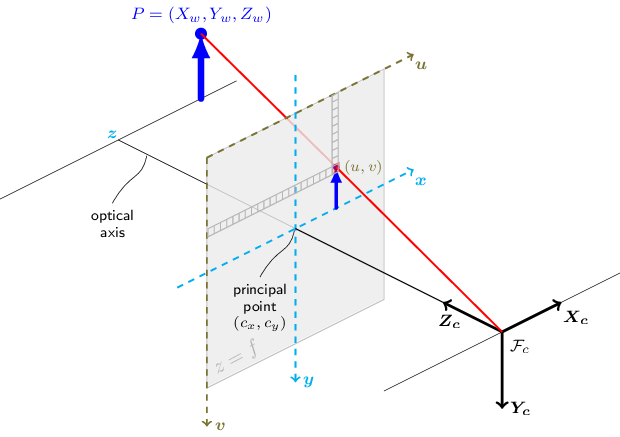
\includegraphics[width=0.5\linewidth]{pinhole_model}
            \caption{Пинхол модель камеры; principal point --- центр изображения, проекция начала координат на плоскость изображения}\label{pic:pinhole_model}
        \end{figure}

        Экран в данной модели может располагаться как между объектом и центром проекции (как показано на рисунке \ref{pic:pinhole_model}), так и за центром проекции. В последнем случае изображение оказывается перевёрнутым.

        \subsection{Условные обозначения}
            \noindent $ f $ --- фокусное расстояние камеры в пиксельной мере
            
            $ u,\,v $ --- горизонтальная и вертикальная координаты соответственно в плоскости изображения (пиксели) 
            
            $ u_0,\,v_0 $ --- координата центра изображения
%            $\Delta u $ --- отклонение лазера от оптического центра на изображении по горизонтальной оси\\
%            $\Delta v$ --- отклонение лазера от оптического центра на изображении по вертикальной оси\\
            
        \subsection{Модель в системе координат принтера}
            Первый расчёт производится в системе координат прототипа. Он основывается на реальных размерах сборки и отражает реальную конструкцию модуля сканирования. В данном варианте расчёта предполагается, что стол -- рабочая поверхность -- находится в плоскости $ XY $, лазер излучает перпендикулярно столу и камера имеет поворот только вокруг оси $ Y $. При этом считается, что лазер не имеет поворота вокруг своей оси.

            Похожий метод расчёта используется в работе Machine vision system for curved surface inspection\cite{Lee2000}.

            \begin{figure}[!ht]\label{pic:first_model}
                \centering
                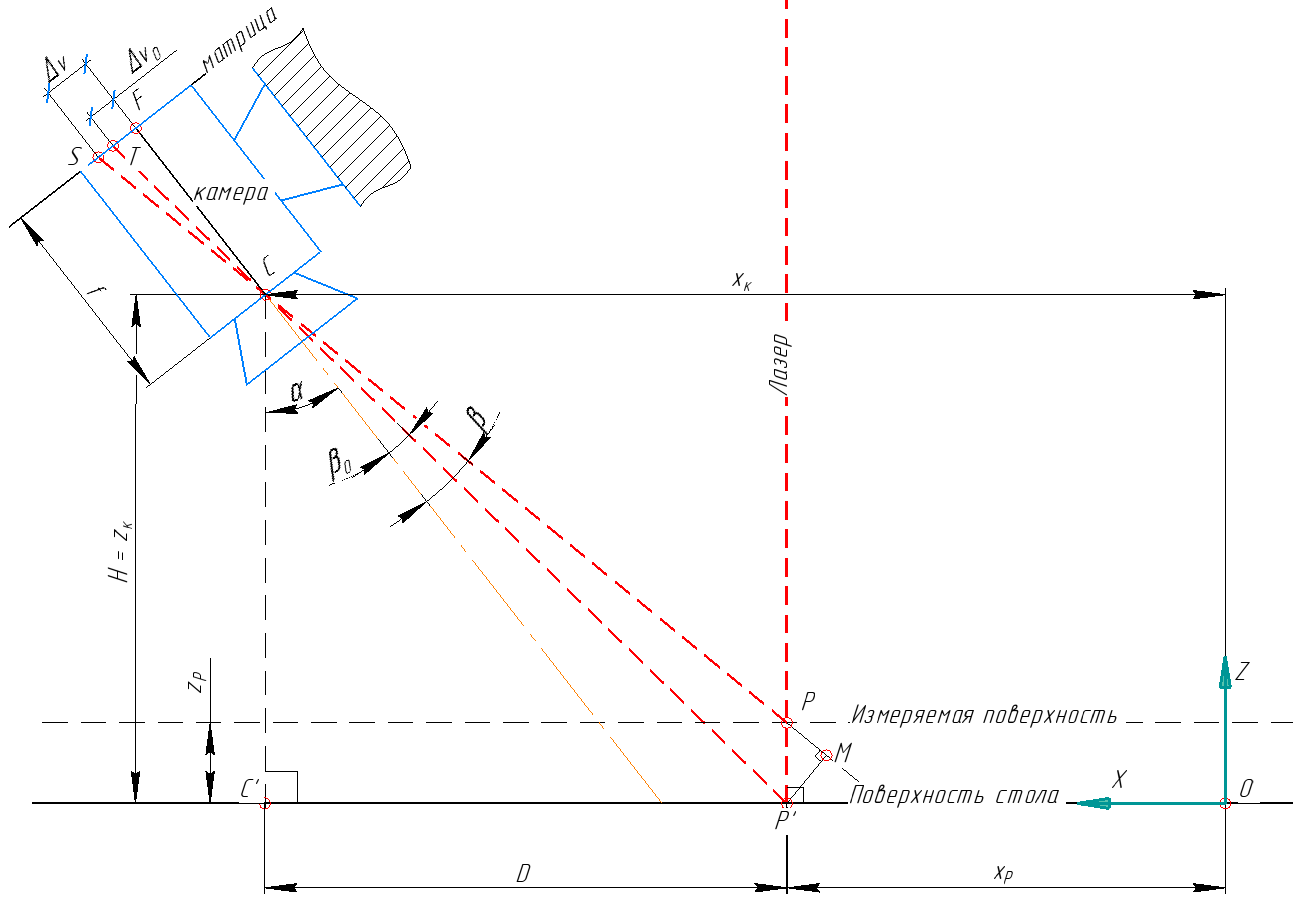
\includegraphics[width=0.75\linewidth]{first_model_xz}
                \caption{Расчёт в системе координат прототипа}
            \end{figure}
            
            \sloppy Необходимо найти уравнения описывающие зависимость координат $ \left(x_P,\,y_P,\,z_P\right) $ точки $ P $ от координат проекции этой точки на плоскость изображения $ \left(u_P, v_P\right) $. Из $ \triangle PP'M $ видно, что
            \begin{equation}
                z_P = \dfrac{P'M}{\cos\angle PP'M}
            \end{equation}
            Далее из $ \triangle CP'M $ очевидно
            \begin{equation}
                P'M = CP'\sin\left(\beta - \beta_0\right)
            \end{equation}
            где $ \beta $ -- произвольный угол падения луча лазера на матрицу,\\
            $\beta_0$ -- угол падения луча лазера отражённого от поверхности стола на матрицу.
            
            Рассмотрев $ \triangle CP'C' $ можно увидеть, что
            \begin{equation}
                CP' = \dfrac{H}{\cos\left(\alpha + \beta_0\right)}
            \end{equation}
            Подставляя последовательно полученные равенства друг в друга получаем следующее уравнение
            \begin{equation}
                z_P = H\dfrac{\sin\left(\beta - \beta_0\right)}{\cos\left(\alpha + \beta_0\right)\cos\angle PP'M}
            \end{equation}
            нетрудно показать, что
            \begin{equation}
                \cos\angle PP'M = \sin\left(\alpha + \beta\right)
            \end{equation}
            В итоге приходим к уравнению координаты $ z $ точки $ P $, выраженной через углы падения луча лазера на матрицу камеры.
            \begin{equation}
                z_P = H\dfrac{\sin\left(\beta - \beta_0\right)}{\cos\left(\alpha + \beta_0\right)\sin\left(\alpha + \beta\right)}
            \end{equation}
            Расстояние точки $ P $ от камеры при данном методе расчёта константа на всём протяжении линии лазера в виду конструкции и равно расстоянию между камерой и лазером $ C'P' = D $
            \begin{equation}
                D = H\tg\left(\alpha + \beta_0\right)
            \end{equation}
            тогда координата $ x_P $ выражается следующим соотношением
            \begin{equation}
                x_P = x_\text{к} - D = x_\text{к}- H\tg\left(\alpha + \beta_0\right)
            \end{equation}
            Для вывода уравнения координаты $ y_P $ необходимо рассмотреть модуль в проекции на плоскость $ ZY $
            \begin{figure}[H]
                \centering
                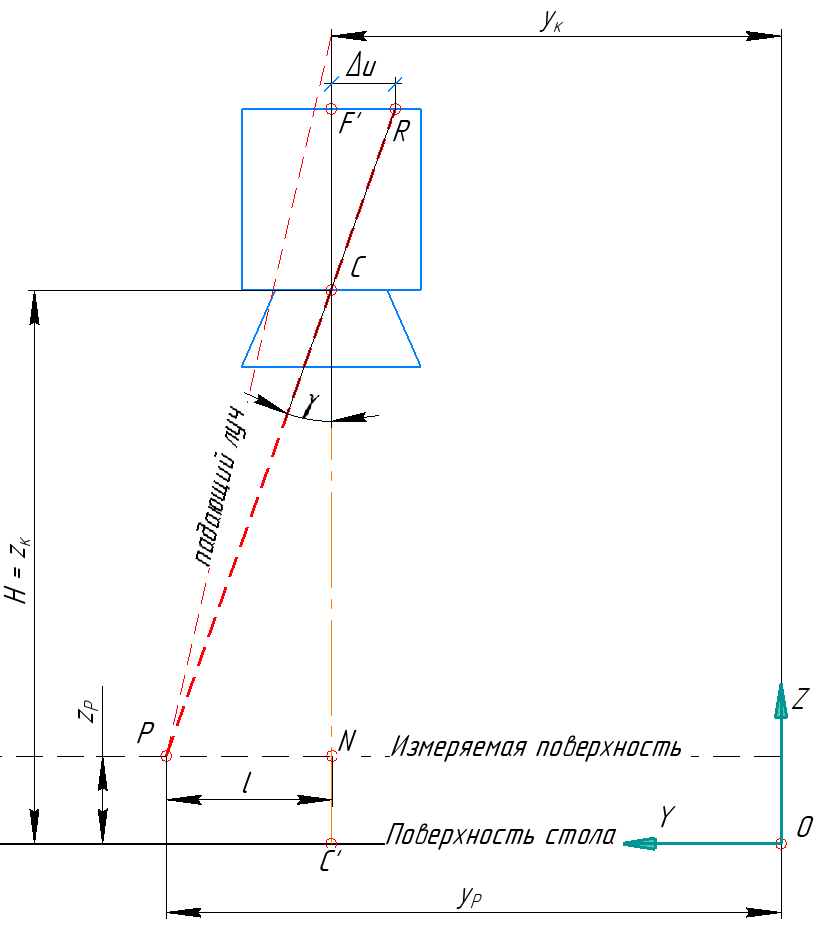
\includegraphics[width=0.5\linewidth]{first_model_yz}
                \caption{Проекция на плоскость $ ZY $}
            \end{figure}
            
            При выводе важно помнить, что данный вид -- проекция.
            Из чертежа очевидно, что 
            \begin{equation}
                y_P = y_\text{к} + l
            \end{equation} 
            Из $ \triangle CPN $ легко вывести $ l $
            \begin{equation}
                l = CN\tg\gamma
            \end{equation}
            где $ \gamma $ -- угол падения луча лазера на матрицу в данной проекции. Поскольку $ CN = H - z_P $ можно записать
            \begin{equation}
                y_P = y_\text{к} + (H - z_P)\tg\gamma
            \end{equation}
            Для вывода углов падения $ \beta $ и $ \beta_0 $ рассмотрим $ \triangle CSF$ и $ \triangle CTF $. Очевидно, что
            \begin{equation}
                \begin{aligned}
                    \tg\beta &= \dfrac{\Delta v}{f}\\
                    \tg\beta_0 &= \dfrac{\Delta v_0}{f}
                \end{aligned}
            \end{equation}
            где $ \Delta v = v_P - v_0 $ -- расстояние в пикселях от точки падения луча лазера на матрицу до центра изображения; \\
            $ \Delta v_0 = v_{P0} - v_0 $ -- аналогичное расстояние для луча лазера, отражённого от поверхности стола.
            
            Рассмотрев $ \triangle CF'R $ получим значение угла падения в проекции $ ZY $
            \begin{equation}
                \tg\gamma = \dfrac{\Delta u}{CF'} = \dfrac{\Delta u}{f\cos\alpha}
            \end{equation}
            где $ CF' = f\cos\alpha $ -- проекция фокусного расстояния на плоскость $ ZY $.
            Из полученных равенств легко найти значения углов, поскольку величины $ \Delta u $ и $ \Delta v $ известны из изображения с камеры.
            
            Таким образом приходим к следующим уравнениям
            \begin{equation}\label{eq:first_model}
                \left\{
                    \begin{aligned}
                        x_P &= x_\text{к}- H\tg\left(\alpha + \beta_0\right)\\
                        y_P &= y_\text{к} + (H - z_P)\dfrac{\Delta u}{f\cos\alpha}\\
                        z_P &= H\dfrac{\sin\left(\beta - \beta_0\right)}{\cos\left(\alpha + \beta_0\right)\sin\left(\alpha + \beta\right)}
                    \end{aligned}
                \right.
            \end{equation}

            Преимущества этой модели:
            \begin{itemize}
                \item $ H $ можно измерять напрямую
                \item рассчитанные значения координат соответствуют системе прототипа
                \item отражает реальную конструкцию сканера
                \item координата $ x $ -- константа относительно камеры
            \end{itemize}
            
            Недостатки:
            \begin{itemize}
                \item много тригонометрических преобразований
                \item при изменении высоты камеры необходимы новые замеры
                \item большое количество допущений, как следствие много возможностей для ошибок
            \end{itemize}

        \subsection{Модель в системе координат камеры}
            Второй расчёт производится в системе координат связанной с камерой. Он основывается на теоретических величинах и происходит в два этапа. Первый -- расчёт координат относительно камеры, второй -- преобразование полученных координат в систему прототипа. В этом расчёте принято допущение, что лазер не имеет поворота вокруг своей оси, все остальные компоненты могут располагаться произвольно.
            
            Для преобразования между двумя системами координат необходимо знать матрицу поворота системы камеры относительно системы прототипа. С помощью пакета opencv можно полностью определить положение камеры в пространстве используя шахматный паттерн\cbox{ссылка на туториал опенсв}.

            Введём следующие определения:\\
            \textit{Рабочая плоскость} --- плоскость перпендикулярная оптической оси камеры и проходящая через точку пересечения оптической оси камеры и луча лазера\\
            \textit{Измеряемая плоскость} --- плоскость, до которой измеряется расстояние 

            \begin{figure}[H]
                \centering
                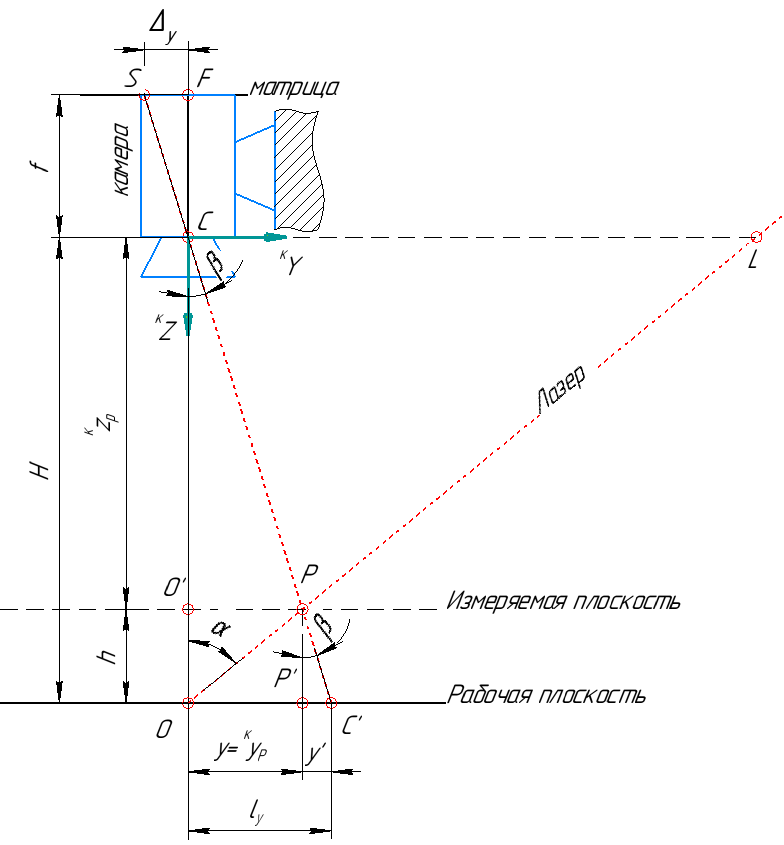
\includegraphics[width=0.75\linewidth]{second_model}
                \caption{Расчёт в системе координат камеры;
                         $O$ --- точка пересечения оптической оси камеры и луча лазера (плоскости свечения лазера);
                         $C$ --- оптический центр камеры, начало координат СК камеры;
                         $P$ --- точка пересечения луча лазера и измеряемой плоскости;
                         $P'$ --- проекция точки $ P $ на рабочую плоскость;
                         $h$ --- высота измеряемой плоскости над рабочей плоскостью;
                         $l_x,\,l_y$ --- кажущиеся координаты измеряемой точки;
                         $x,\,y$ --- реальные координаты измеряемой точки;
                         $x',\,y'$ --- разность кажущейся и реальной координаты измеряемой точки}
                 \label{pic:second_model}
                 \cbox{ИСПРАВИТЬ ЧЕРТЁЖ}
            \end{figure}
            
            На рисунке \ref{pic:second_model} обозначены следующие размеры:\\
            $ H $ -- рабочая высота, расстояние от оптического центра камеры до рабочей плоскости.\\
            $ \alpha $ -- угол между осями камеры и лазера.
            
            \sloppy Необходимо найти уравнения описывающие зависимость координат $ \left(\kxp,\,\kyp,\,\kzp\right) $ точки $ P $ в системе координат камеры от координат проекции этой точки на плоскость изображения $ \left(u_P,\,v_P\right) $. 
            Из чертежа очевидно, что 
            \begin{equation}
                \kzp = H - h,
            \end{equation} 
            где $ h $ -- высота измеряемой плоскости над рабочей. 
            Рассмотрим треугольники $ \triangle OPC $, $ \triangle OPP' $, $\triangle PCP' $.
            Видно что 
            \begin{equation}
                l_y = y + y',
            \end{equation}
            где $ l_y $ -- кажущаяся координата точки $ P $;\\
            $ y = \kyp $ -- реальная координата точки $ P $;\\
            $ y' $ -- разность реальной и кажущейся координаты.
            Так как $ PP' = h $ можно записать следующее:
            \begin{equation}
                \begin{aligned}
                    y &= h \tg\alpha\\
                    y' &= h \tg\beta
                \end{aligned}
            \end{equation}
            где $ \beta $ -- угол при вершине $ P $ в треугольнике $ \triangle PCP' $, $ \alpha $ -- угол между оптической осью камеры и осью лазера.
            Также из треугольника $ \triangle COC' $ ясно
            \begin{equation}
                l = H \tg\beta
            \end{equation}
            следовательно
            \begin{equation}
                H\tg\beta = h\left(\tg\alpha+\tg\beta\right)
            \end{equation}
            Зная, что $ h = H - \kzp $ получаем
            \begin{equation}
                \kzp = H \dfrac{\tg\alpha}{\tg\alpha + \tg\beta}
            \end{equation}
            
            Из треугольника $ \triangle CF\cbox{\text{НЕТ БУКВЫ}} $ находим
            \begin{equation}
                \tg\beta = \dfrac{\Delta v}{f},
            \end{equation}
            где $ \Delta v = v_P - v_0 $, $ f $ -- фокусное расстояние камеры.
            В итоге получаем
            \begin{equation}
                \kzp = H \dfrac{\tg\alpha}{\tg\alpha + \frac{\Delta v}{f}}
            \end{equation}
            Далее из $ \triangle C\cbox{\text{НЕТ БУКВЫ}}P $ очевидно, что
            \begin{equation}\label{eq:kyp}
                \kyp = \kzp \tg\beta = H \dfrac{\tg\alpha\frac{\Delta v}{f}}{\tg\alpha + \frac{\Delta v}{f}}
            \end{equation}
            аналогично для $ \kxp $
            \begin{equation}\label{eq:kxp}
                \kxp =\kzp \tg\gamma = H \dfrac{\tg\alpha\frac{\Delta u}{f}}{\tg\alpha + \frac{\Delta v}{f}}
            \end{equation}
            где $ \tg\gamma = \dfrac{\Delta u}{f} $ -- угол падения луча лазера на матрицу в плоскости $ XZ $, $ \Delta u = u_P-u_0 $.
            
            В результате для системы координат камеры получаем:
            \begin{equation}\label{eq:second_model}
                \left\{
                    \begin{aligned}
                        \kxp = H\frac{\tg\alpha\frac{\Delta u}{f}}{\tg\alpha+\frac{\Delta v}{f}}\\
                        \kyp = H\frac{\tg\alpha\frac{\Delta v}{f}}{\tg\alpha+\frac{\Delta v}{f}}\\
                        \kzp = H\frac{\tg\alpha}{\tg\alpha+\frac{\Delta v}{f}}
                    \end{aligned}
                \right.
            \end{equation}
            
            Для перевода в систему прототипа:
            \begin{equation}\label{eq:coord_world}
                \begin{pmatrix}
                    x_P\\y_P\\z_P
                \end{pmatrix}
                =
                R
                \begin{pmatrix}
                    \kxp\\ \kyp\\ \kzp
                \end{pmatrix}
                +
                \begin{pmatrix}
                    x_\text{к}\\y_\text{к}\\z_\text{к}
                \end{pmatrix}
            \end{equation}
            
            Преимущества модели:
            \begin{itemize}
                \item отсутствие тригонометрии в расчётах координат
                \item параметры $ H $ и $ \alpha $ фиксированы
                \item меньшее количество допущений
            \end{itemize}
            
            Недостатки модели:
            \begin{itemize}
                \item сложно прямо измерить $ H $ и $ \alpha $, необходим теоретический расчёт
                \item необходима матрица поворота камеры
            \end{itemize}
            
        \subsection{Выбор модели}
            Сравнивая расчёты мы видим, что недостатки второго менее серьёзны чем первого, а также что второй расчёт не имеет недостатков первого. В частности расчёт в системе координат камеры упрощает эксплуатацию модуля, т.к. отсутствует необходимость повторных измерений параметров при изменении положения внешних по отношению к модулю элементов (например, перемещение стола). Также меньшее количество допущений для второй модели позволяет добиться более точных результатов не имеющих пространственных искажений (например, растяжение сцены), которые могут возникать в следствии дополнительного неучтенного наклона камеры.
            Таким образом более выгодным вариантом расчёта является вторая модель.
            
            \sloppy Использование этой модели требует дополнительных предварительных расчётов, для использования, а именно -- расчёт положения камеры относительно системы координат принтера и расчёт параметров модуля $ H $ и $\alpha$. Расчёт положения камеры -- матрицы поворота $ R $ и координат $ \left(x_\text{к},\,y_\text{к},\,z_\text{к}\right) $ -- можно произвести средствами библиотеки OpenCV используя специальный шахматный паттерн (подробнее в главе \ref{chap:algorithms}). Для расчёта параметров модуля необходимо вывести соответствующий расчёт на основе уравнений \ref{eq:second_model} \ref{eq:coord_world}, что делается в разделе \ref{sec:scan_calib}.

    \section{Оценка дискретности}\label{sec:error}
        Для удовлетворения характеристик, заданных ТЗ необходимо выбрать подходящие значения параметров $ H $ и $\alpha$. Эти параметры определяют разрешающую способность сканера и ширину обзора камеры. Разрешающая способность камеры -- разность определяемых высот между соседними пикселями.
        
        Для простоты примем, что рабочая плоскость совпадает со столом и лазер излучает перпендикулярно столу. Таким образом $\alpha$ становится углом наклона камеры от вертикали. Для данной оценки и последующего применения результатов примем $ H $ равной высоте камеры над столом. Также, поскольку основным изделием является печенье, нас в первую очередь интересует диапазон высот объектов 5-20 мм.
        \cbox{разделить на а и б графики}
        \begin{figure}[H]
            \centering
            \begin{subfigure}{\linewidth}
                \centering
                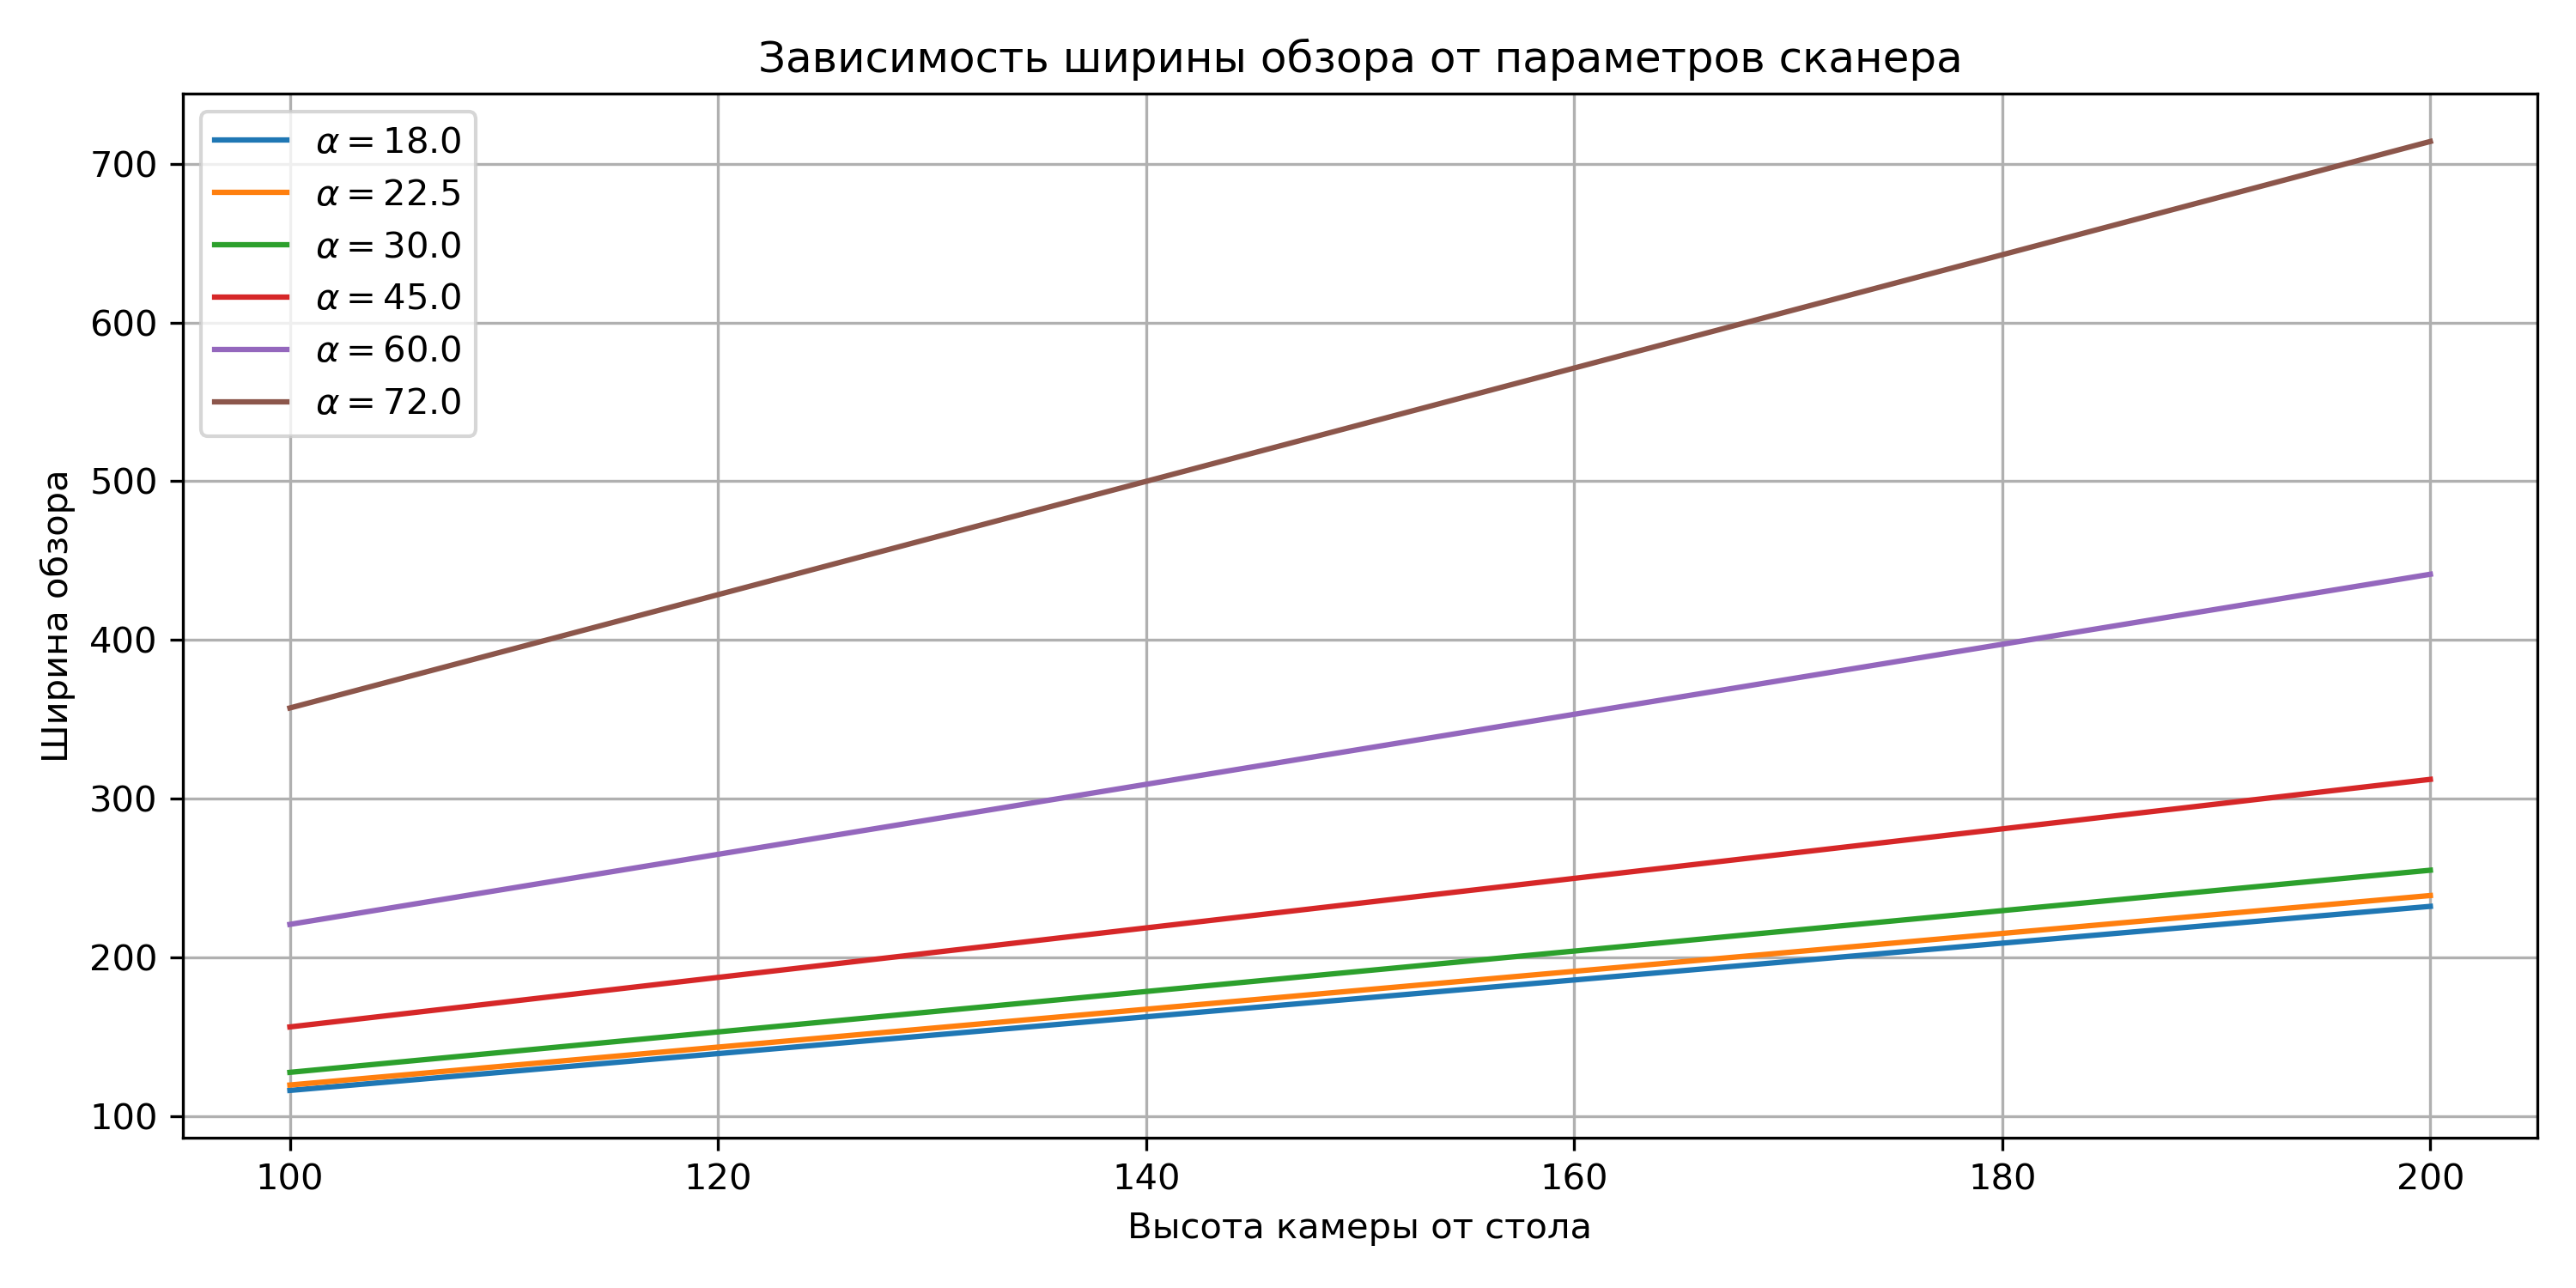
\includegraphics[width=\linewidth]{view_width_1}
                \caption{от $ H $ с параметром $ \alpha $}
            \end{subfigure}
            \begin{subfigure}{\linewidth}
                \centering
                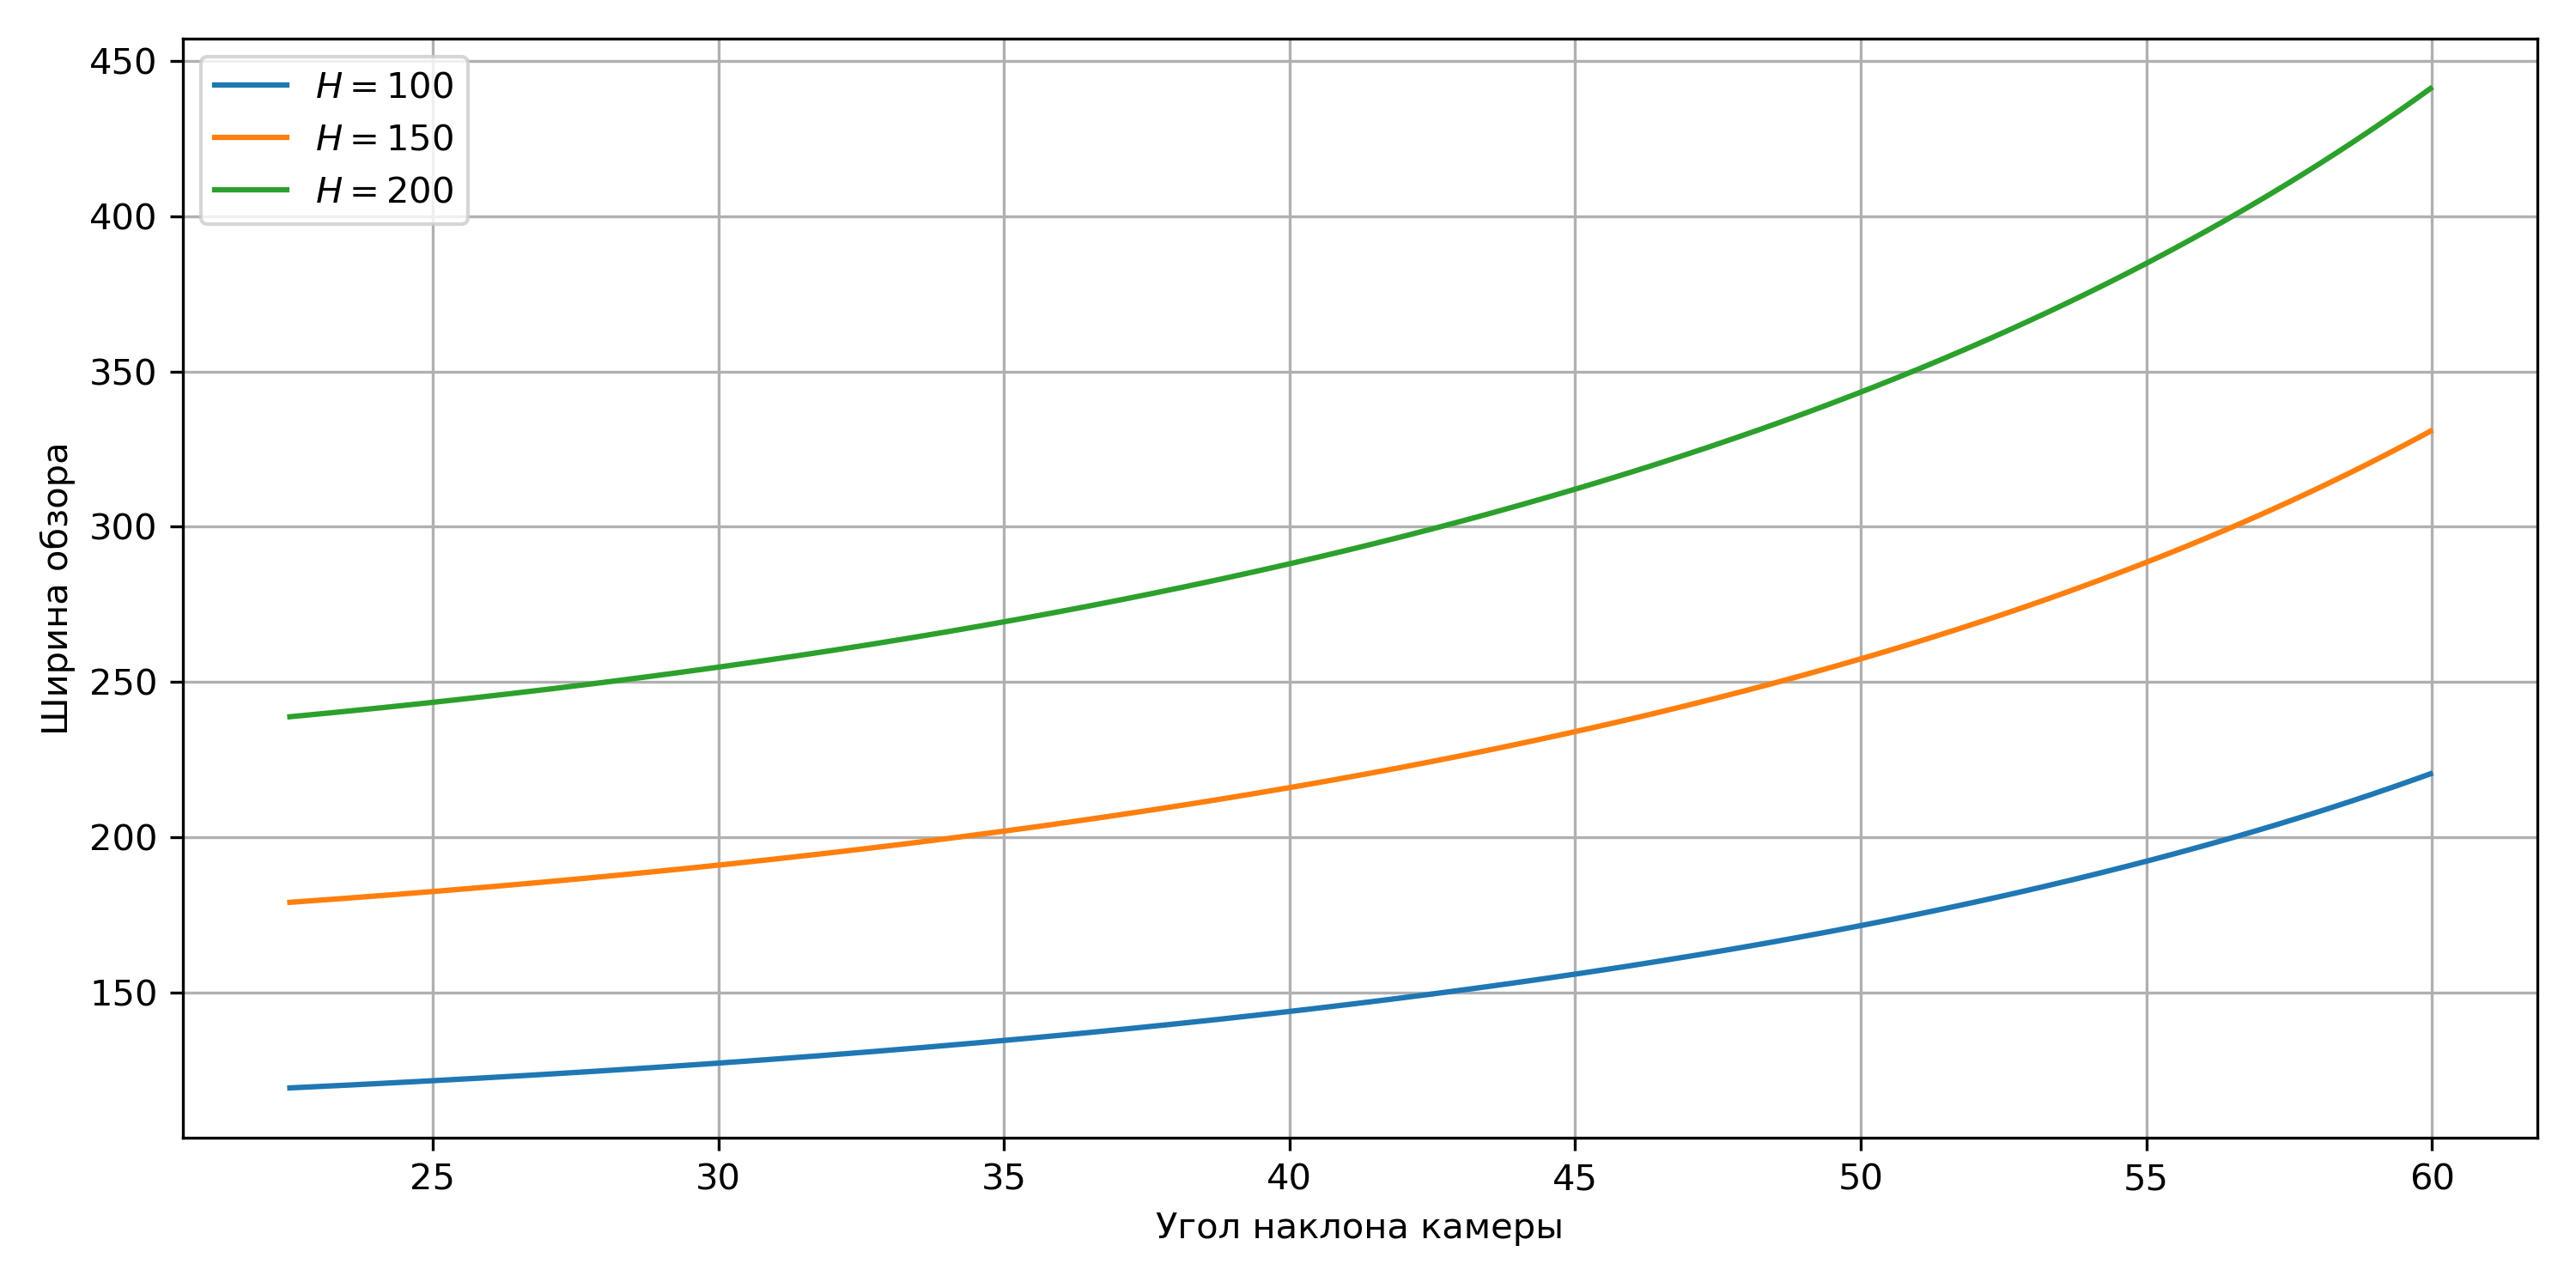
\includegraphics[width=\linewidth]{view_width_2}
                \caption{от $ \alpha $ с параметром $ H $}
            \end{subfigure}
            \caption{Зависимость ширины обзора камеры от параметров сканера}
            \label{pic:view_width}
        \end{figure}
        Сначала рассмотрим рисунок \ref{pic:view_width} на котором изображена зависимость ширины обзора при разных параметрах сканера. На графике линии показывают ширину обзора по центру кадра, так как мы предполагаем, что рабочая плоскость располагается в плоскости стола. Видно, что чем больше высота над столом $ H $ и угол от вертикали $ \alpha $, тем больше ширина обзора. Необходимая ширина обзора по ТЗ равна 200 мм. Этот рисунок поможет выбрать оптимальное значение при исследовании графиков изображённых на следующем рисунке \ref{pic:discretion}.
        \begin{figure}[H]
            \centering
            \begin{subfigure}{\linewidth}
                \centering
                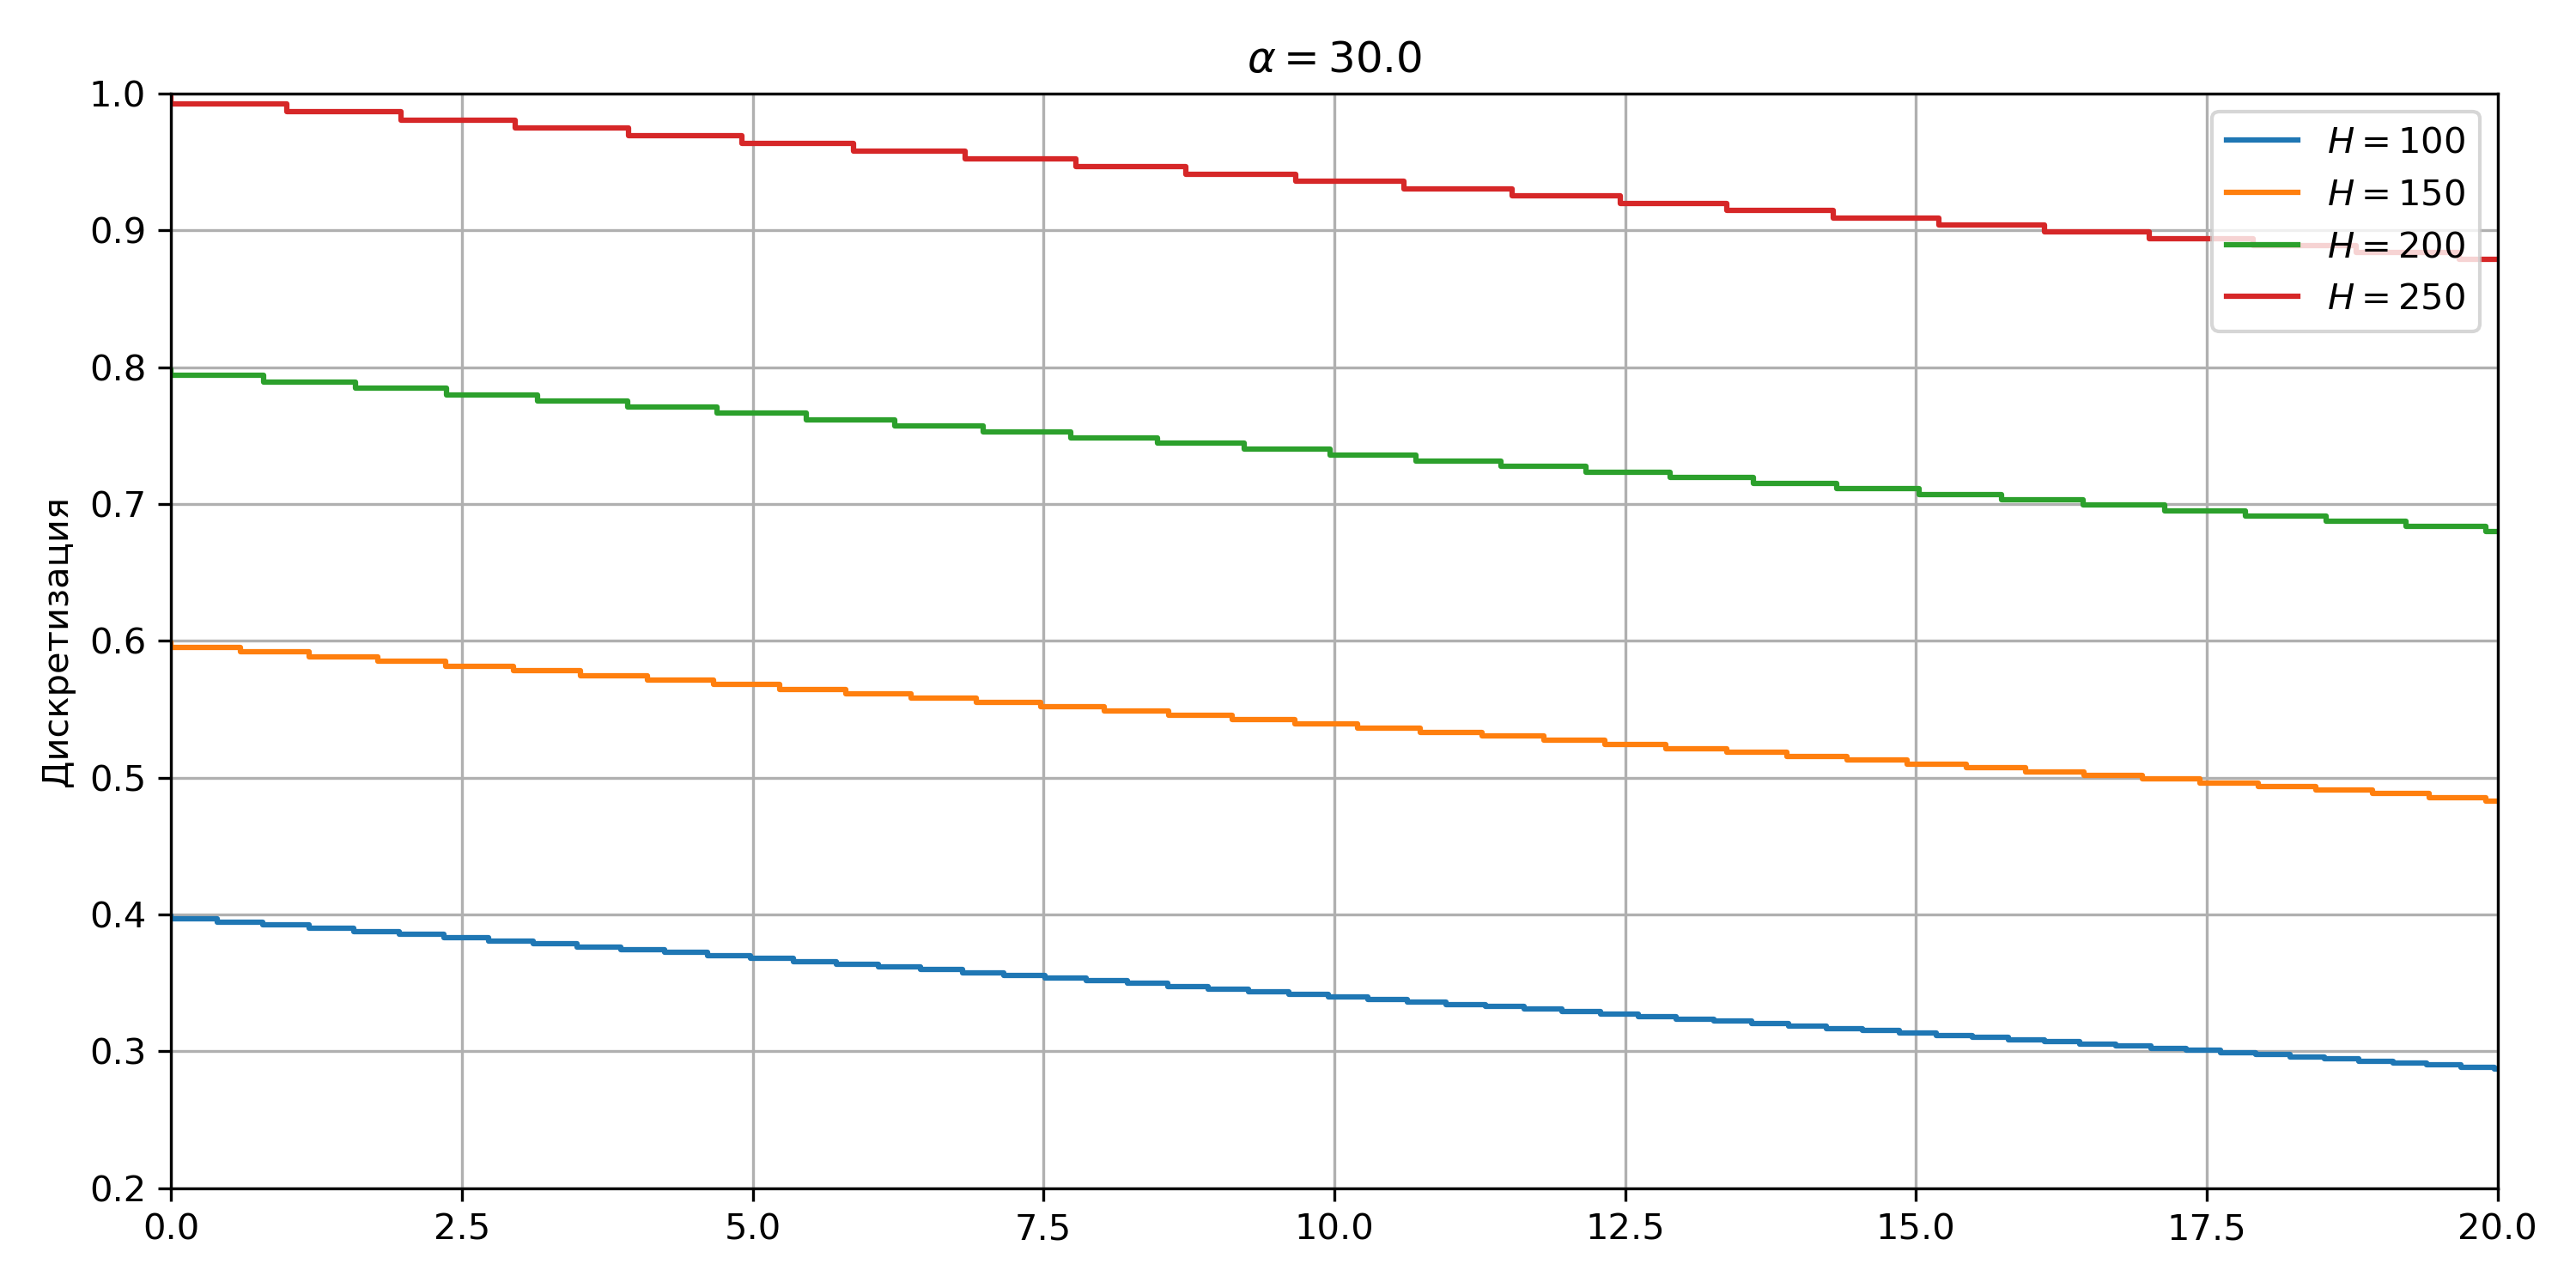
\includegraphics[width=\linewidth]{discretion_1}
                \caption{$ \alpha = 30\degs $, разные $ H $}
            \end{subfigure}
            \begin{subfigure}{\linewidth}
                \centering
                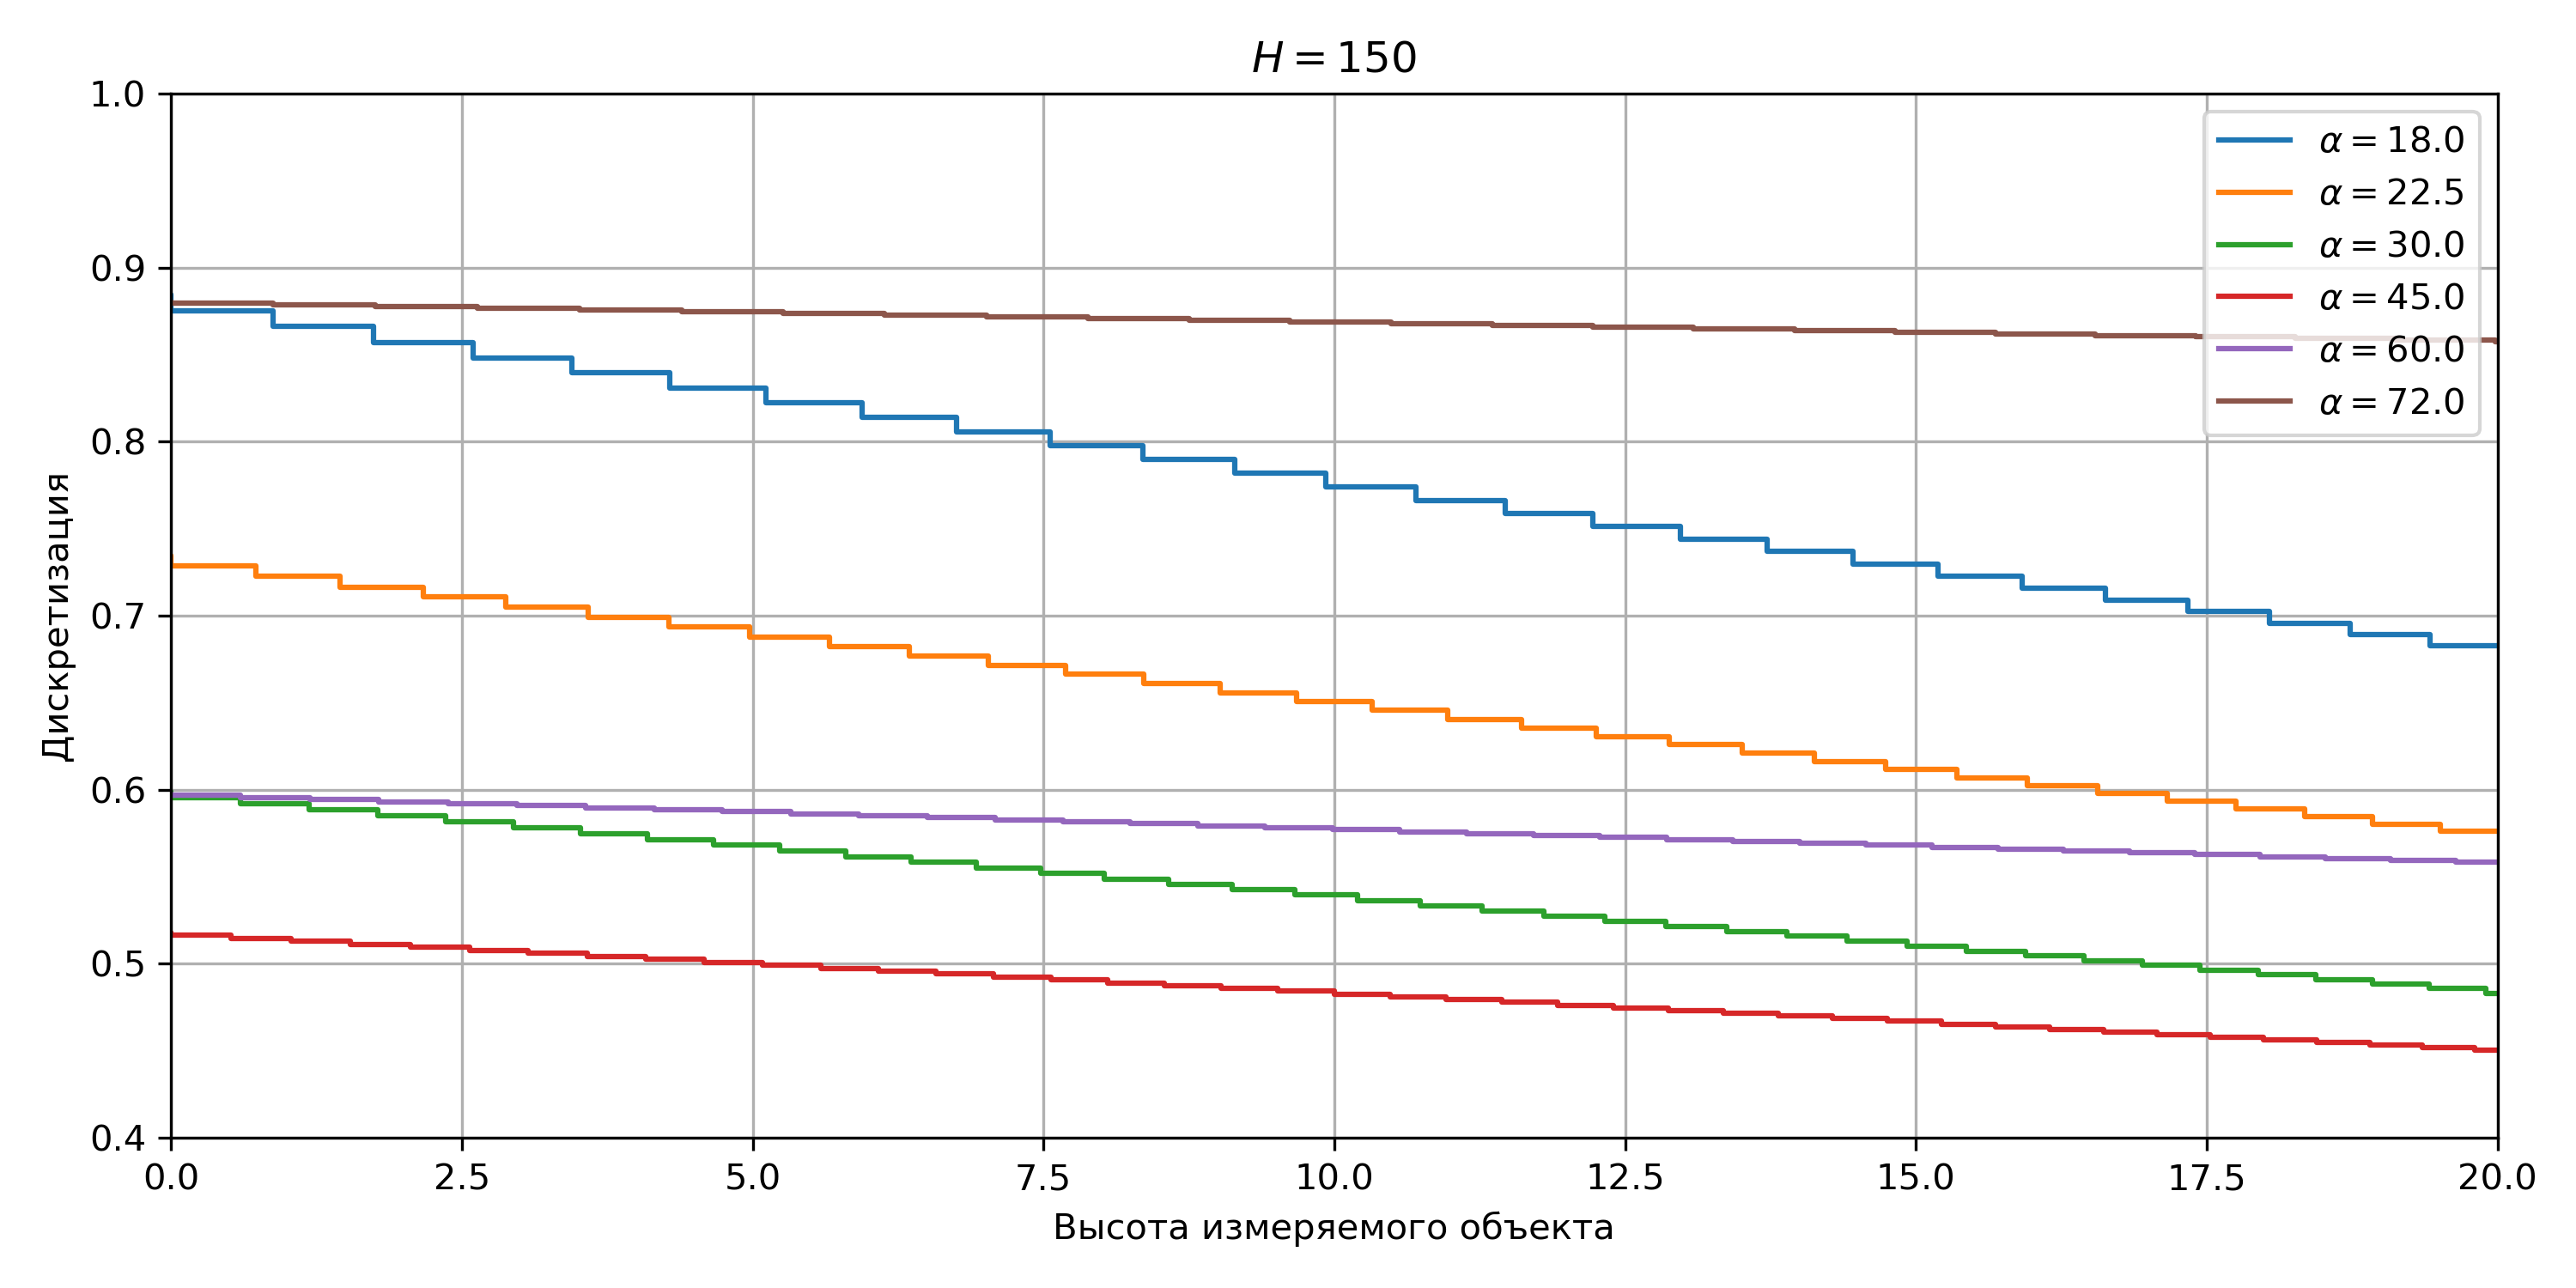
\includegraphics[width=\linewidth]{discretion_2}
                \caption{$ H = 150 $, разные $ \alpha $}
            \end{subfigure}
            \caption{Зависимость дискретизации от параметров сканера}
            \label{pic:discretion}
        \end{figure}
        По графикам на рисунке \ref{pic:discretion} видно, что дискретизация растёт с увеличением высоты камеры над столом, что логично т.к. при этом на один пиксель приходится большее расстояние. От угла же дискретизация зависит иначе - чем дальше угол от $ 45\degs $, тем  она больше. Требуемая точность системы $ \pm 0.5\text{ мм} $, таким образом дискретность должна быть не больше этого значения. Видно, что наиболее выгодные значения параметров лежат в интервалах $ 130 \text{ мм} \le H \le 150 \text{ мм} $; $ 30\degs \le \alpha \le 60\degs $. 
        При параметрах из данного диапазона одновременно достигается заданная точность и ширина обзора.
        При этом здесь рассматривается случай, когда лазер на изображении находится с точностью до пикселя, однако итоговый модуль использует алгоритм нахождения лазера с субпиксельной точностью, что ещё больше снижает дискретизацию и позволяет компенсировать ошибки возникающие при сборке модуля или невозможности использовать идеальные параметры.

    \section{Калибровка сканера}\label{sec:scan_calib}
        Для калибровки сканера -- расчёта параметров $ H $ и $\alpha$ -- необходимо вывести уравнения, в которых используя известные высоты эталонов можно рассчитать искомые величины.
        Для этого воспользуемся уравнением координаты $ \kzp $ из \ref{eq:second_model}
        \begin{equation}
            \kzp = H\frac{\tg\alpha}{\tg\alpha+\frac{\Delta v}{f}}
        \end{equation}
        Имея два таких уравнения для разных высот $ \kz{i} $ и $ \kz{k} $ и соответствующих им разностей пикселей $ \Delta v_i $ и $ \Delta v_k $ получаем следующую систему уравнений
        \begin{equation}
            \left\{
                \begin{aligned}
                    \kz{i} &= H\frac{\tg\alpha}{\tg\alpha+\frac{\Delta v_i}{f}}\\
                    \kz{k} &= H\frac{\tg\alpha}{\tg\alpha+\frac{\Delta v_k}{f}}
                \end{aligned}
            \right.
        \end{equation}
        разделив $ \kz{i} $ на $ \kz{k} $ получаем уравнение с одной неизвестной $ \tg\alpha $
        \begin{equation}
            \dfrac{\kz{i}}{\kz{k}} = \dfrac{\tg\alpha + \frac{\Delta v_k}{f}}{\tg\alpha+\frac{\Delta v_i}{f}}
        \end{equation}
        проделав небольшие преобразования приходим к окончательному уравнению для $ \tg\alpha $
        \begin{equation}
            \tg\alpha = \dfrac{\kz{k}\frac{\Delta v_k}{f} - \kz{i}\frac{\Delta v_i}{f}}{\kz{i} - \kz{k}}
        \end{equation}
        Конкретное значение угла в данном случае неважно поскольку в расчётах используется именно $ \tg\alpha $, поэтому можно оставить так.
        Подставляя полученное равенство в любое уравнение в системе после преобразований получаем уравнение для $ H $
        \begin{equation}
            H = \kz{i}\kz{k}\dfrac{\Delta v_k-\Delta v_i}{\kz{k}\Delta v_k - \kz{i}\Delta v_i}
        \end{equation}
        Таким образом получаем систему уравнений, позволяющую рассчитать параметры сканера зная координаты двух точек $ \kz{i} $ и $ \kz{k} $ в системе камеры и соответствующих им разностей координат в плоскости изображения.
        \begin{equation}\label{eq:calib1}
            \left\{
                \begin{aligned}
                    \tg\alpha &= \dfrac{\kz{k}\frac{\Delta v_k}{f} - \kz{i}\frac{\Delta v_i}{f}}{\kz{i} - \kz{k}}\\
                    H &= \kz{i}\kz{k}\dfrac{\Delta v_k-\Delta v_i}{\kz{k}\Delta v_k - \kz{i}\Delta v_i}
                \end{aligned}
            \right.
        \end{equation}
        Или можно переписать данную систему через углы падения луча лазера на матрицу $ \beta $ и получить следующую систему
        \begin{equation}\label{eq:calib2}
            \left\{
                \begin{aligned}
                    \tg\alpha &= \dfrac{\kz{k}\tg\beta_k - \kz{i}\tg\beta_i}{\kz{i} - \kz{k}}\\
                    H &= \kz{i}\kz{k}\dfrac{\tg\beta_k-\tg\beta_i}{\kz{k}\tg\beta_k - \kz{i}\tg\beta_i}
                \end{aligned}
            \right.
        \end{equation}
        Однако полученная система уравнений зависит от координат в системе камеры, которые сложно измерить на практике. Необходимо привести уравнения к использованию координат из системы принтера. Данные координаты гораздо легче получить, т.к. возможно произвести прямые измерения этих величин. Для перевода координат из системы камеры в систему принтера воспользуемся уравнением \ref{eq:coord_world}. Согласно данному уравнению координата $ z_P $ точки $ P $ в системе принтера выражается следующим образом
        \begin{equation}
            z_P = r_{31}\kxp +r_{32}\kyp+r_{33}\kzp + z_\text{к}
        \end{equation}
        подставляя сюда уравнения \ref{eq:kxp} и \ref{eq:kyp} получаем
        \begin{equation}
            z_P = r_{31}\kzp\tg\gamma +r_{32}\kzp\tg\beta+r_{33}\kzp + z_\text{к}
        \end{equation}
        соответственно $ \kzp $ равняется
        \begin{equation}\label{eq:calib_kzp}
            \kzp = \dfrac{z_p - z_\text{к}}{r_{31}\tg\gamma +r_{32}\tg\beta+r_{33}}
        \end{equation}
        
        Таким образом для калибровки необходимо выполнить следующее
        \begin{enumerate}
            \item Измерить координату $ z $ минимум пары эталонов в системе принтера
            \item Для каждого эталона определить $ \Delta v $ или $ \tg\beta $
            \item Перевести координаты в систему камеры подставив в уравнение \ref{eq:calib_kzp}
            \item Подставить полученные координаты и соответствующие углы в уравнение \ref{eq:calib1} или \ref{eq:calib2}
        \end{enumerate}
        Для лучшей точности рекомендуется выбирать пары эталонов с наибольшей разницей в высоте, а также проводить множество расчётов с различными парами эталонов для усреднения результатов и минимизации ошибки измерений.